
% \mainmatter
% \cleartoleftpage

% \thispagestyle{empty}
% \vspace*{\fill}
% \newpage

\onehalfspacing
\pagenumbering{arabic}
\setcounter{page}{1}
\pagestyle{scrheadings}

\section{Einleitung}

In der heutigen Zeit nimmt die Popularität und Anwendungsmöglichkeit künstlicher Intelligenz immer stärker zu \autocite[S.1]{Boutaba.2018}
Dies liegt einerseit an der Explosion erstellter und öffentlich zugänglicher Daten, aber auch anderseits an der vorgeschrittenen Forschung im Bereich \gls{ml}, welcher als Teilbereich der \gls{ki} fungiert. Zudem tragen die erweiterten \enquote{computing capabilities} \autocite[S.1]{Boutaba.2018} zu neuen Möglichkeiten der Applikation von \gls{ml} bei. Ein komplexeres und fortgeschrittenes \gls{ml}-Thema ist das \textit{Ensemble Learning}. Im folgenden soll dieses komplexe Thema hinsichtlich der allgemeinen Definition, der verschiedene Methodenansätze, der Aggregationsmöglichkeiten und der Anwendungsbereiche dargestellt und erläutert werden. Unter \textit{Ensemble Learning} versteht man ein \enquote{multiple classifier system}\autocite[S.182]{Zhou.2021}, welches auch \enquote{committee-based learning}\autocite[S.15]{Zhou.2012} genannt wird. Hierzu werden individuelle Lernalgorithmen zunächst auf bestimmte Art und Weise trainiert und folgend mit Hilfe einer bestimmten Kombinationstechnik aggregiert. Es gibt zwei verschiedene Arten, den homogenen und heterogenen Ensembles, zwischen denenen unterschieden werden kann. Homogen bedeutet, dass alle individuellen \glspl{baselearner}\autocite[S.182]{Zhou.2021} auf den gleichen Lernalgorithmen basieren, wodurch hingegen heterogene Ensembles auf die Verwendung unterschiedlicher \textit{base learners} und somit Lernalgorithmen aufbauen. Werd ein heterogenes Ensemble betrachtet, so spricht man jedoch nicht mehr von \textit{base learners}, sondern von \enquote{component learners}\autocite[S.15]{Zhou.2012}. Ein Vorteil bei der Anwendung von \textit{Ensemble Learning}-Methoden ist die Verbesserung des Verallgemeinerungsfähigkeit, besser bekannt unter der \enquote{generalization ability}\autocite[S.15]{Zhou.2021}, wobei damit die Fähigkeit gemeint ist, wie gut der Lernalgorithmus nicht nur die Trainigsdaten, sondern auch noch nie zuvor gesehene Testdaten generalisieren kann.

\section{Bagging}
Da die Verallgemeinerungsfähigkeit der Ensembles von der Unabhängigkeit der individuellen \textit{base learners} abhängt und eine strikte Unabhängigkeit leider nicht gewährleistet werden kann, wird versucht, die Lernalgorithmen so unterschiedlich wie möglich voneinander zu erstellen. Dies kann  bereitgestellt werden, indem jeder \textit{base learner} auf einer bestimmten Partition des ganzen, originalen Datensatzes trainiert wird. Dabei muss beachtet werden, dass wenn nicht ausreichend Daten für das Training zur Verfügung stehen, die Partitionen so erstellt werden müssen, dass sie sich in gewissen \glspl{sample} überlappen \autocite[vgl. S.189]{Zhou.2021}. Eine Ensemble Methode die diesen Ansatz verfolgt, ist \textit{Bagging}\autocite[]{Breiman.1996}. \textit{Bagging} ist eine repräsentative Methode des parallelem \textit{Ensemble Learning}'s, die auf dem sogenannten \textit{Bootstrap sampling} basiert. Der Prozess funktioniert folgendermaßen: Gibt es einen Datensatz $D = \{(x_1,y_1), (x_2,y_2), \dots, (x_m,y_m)\}$, wobei $y_i$ dem \gls{label} des Datensamples entsptricht, mit $m$-Samples, dann wird \enquote{randomly}\autocite[S.190]{Zhou.2021} ein Sample aus dem Datensatz kopiert. Dieser Vorgang wird mit \enquote{replacement}\autocite[S.1]{Breiman.1996} ausgeführt, dass heißt, dass eben nur das Sample kopiert wird und sich danach noch immer im originalen Datensatz befindet. Führt man diesen Prozess $T$-mal durch so entstehen dementsprechend auch $T$ Datensatzpartitionen. Die \gls{baselearner} können nun auf den Partitionen trainiert und daraufhin kombiniert werden \autocite[vgl. S.190]{Zhou.2021}.
Eine Übersicht des Verfahren bietet \autoref{fig:bagging}. Der Aspekt des \textit{replacements} wird durch die orangen Samples veranschaulicht, da eigentlich nur ein oranges Samples in $D$ enthalten ist, jedoch durch die \textit{bootstrap sampling}-Methode das orange Sample mehr als einmal in den Bootstrapdatensätzen $\{{D_{B1}, D_{B2}, \dots, D_{BT}\}}$ existieren kann (siehe $D_{B2}, D_{BT}$).

\vspace{4ex}

\begin{figure}[h]
    \centering
    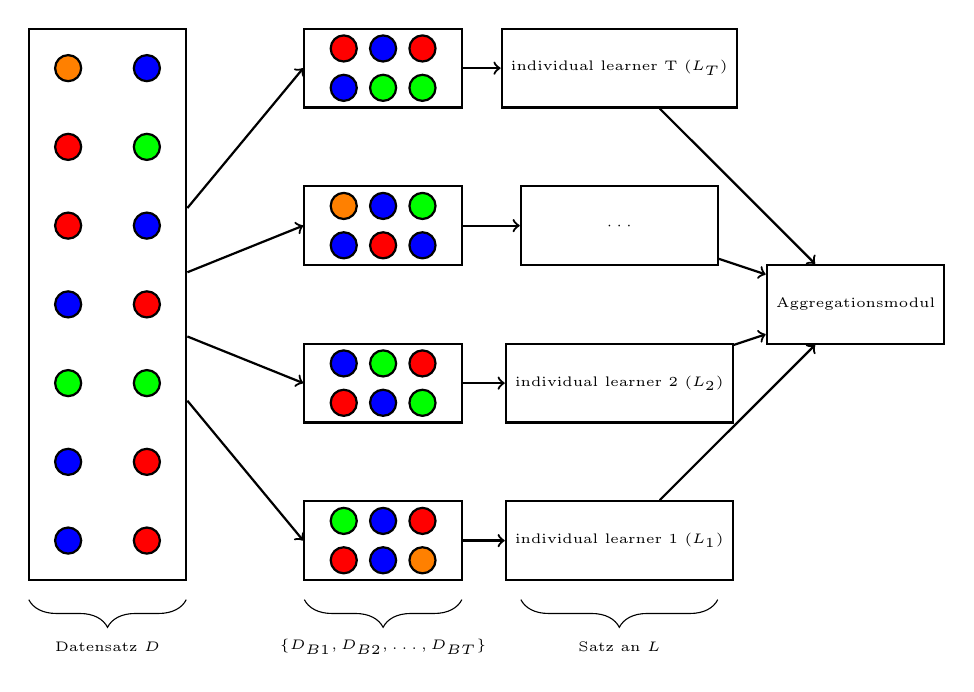
\begin{tikzpicture}
        %original dataset
        \node (dataset) at (-4,3) [draw,thick,minimum width=2cm, minimum height=7cm] {};

        %bootstrapped distribution
        \node (bstp1) at (-0.5,0) [draw,thick,minimum width=2cm,minimum height=1cm] {};
        \node (bstp2) at (-0.5,2) [draw,thick,minimum width=2cm,minimum height=1cm] {};
        \node (bstpdots) at (-0.5,4) [draw,thick,minimum width=2cm,minimum height=1cm] {};
        \node (bstpT) at (-0.5,6) [draw,thick,minimum width=2cm,minimum height=1cm] {};

        %individual learners T
        \node (learner1) at (2.5,0) [draw,thick,minimum width=2.5cm,minimum height=1cm] {\tiny individual learner 1 ($L_1$)};
        \node (learner2) at (2.5,2) [draw,thick,minimum width=2.5cm,minimum height=1cm] {\tiny individual learner 2 ($L_2$)};
        \node (learnerdots) at (2.5,4) [draw,thick,minimum width=2.5cm,minimum height=1cm] {\tiny $\cdots$};
        \node (learnerT) at (2.5,6) [draw,thick,minimum width=2.5cm,minimum height=1cm] {\tiny individual learner T ($L_T$)};

        %combining module
        \node (aggmodule)  at (5.5,3) [draw,thick,minimum width=2cm,minimum height=1cm] {\tiny Aggregationsmodul};

        \draw[->, thick]   (dataset) edge [] node[above]{} (bstp1.west);
        \draw[->, thick]   (dataset) edge [] node[above]{} (bstp2.west);
        \draw[->, thick]   (dataset) edge [] node[above]{} (bstpdots.west);
        \draw[->, thick]   (dataset) edge [] node[above]{} (bstpT.west);

        \draw[->, thick]   (bstp1) edge [] node[above]{} (learner1);
        \draw[->, thick]   (bstp2) edge [] node[above]{} (learner2);
        \draw[->, thick]   (bstpdots) edge [] node[above]{} (learnerdots);
        \draw[->, thick]   (bstpT) edge [] node[above]{} (learnerT);

        \draw[->, thick]   (learner1) edge [] node[above]{} (aggmodule);
        \draw[->, thick]   (learner2) edge [] node[above]{} (aggmodule);
        \draw[->, thick]   (learnerdots) edge [] node[above]{} (aggmodule);
        \draw[->, thick]   (learnerT) edge [] node[above]{} (aggmodule);

        %sample distribution
        \node (sample) at (-3.5,0) [draw,circle,thick,fill=red]{};
        \node (sample) at (-4.5,0) [draw,circle,thick,fill=blue]{};
        \node (sample) at (-3.5,1) [draw,circle,thick,fill=red]{};
        \node (sample) at (-4.5,1) [draw,circle,thick,fill=blue]{};
        \node (sample) at (-3.5,2) [draw,circle,thick,fill=green]{};
        \node (sample) at (-4.5,2) [draw,circle,thick,fill=green]{};
        \node (sample) at (-3.5,3) [draw,circle,thick,fill=red]{};
        \node (sample) at (-4.5,3) [draw,circle,thick,fill=blue]{};
        \node (sample) at (-3.5,4) [draw,circle,thick,fill=blue]{};
        \node (sample) at (-4.5,4) [draw,circle,thick,fill=red]{};
        \node (sample) at (-3.5,5) [draw,circle,thick,fill=green]{};
        \node (sample) at (-4.5,5) [draw,circle,thick,fill=red]{};
        \node (sample) at (-3.5,6) [draw,circle,thick,fill=blue]{};
        \node (sample) at (-4.5,6) [draw,circle,thick,fill=orange]{};

        %bootstrap samples

        %bootstrap samples 1
        \node (samples) at (0,0.25) [draw,circle,thick,fill=red]{};
        \node (sample) at (-1,0.25) [draw,circle,thick,fill=green]{};
        \node (sample) at (0,-0.25) [draw,circle,thick,fill=orange]{};
        \node (sample) at (-1,-0.25) [draw,circle,thick,fill = red]{};
        \node (sample) at (-0.5,0.25) [draw,circle,thick,fill= blue]{};
        \node (sample) at (-0.5,-0.25) [draw,circle,thick, fill=blue]{};

        %bootstrap samples 2
        \node (samples) at (0,2.25) [draw,circle,thick,fill=red]{};
        \node (sample) at (-1,2.25) [draw,circle,thick,fill=blue]{};
        \node (sample) at (0,1.75) [draw,circle,thick,fill=green]{};
        \node (sample) at (-1,1.75) [draw,circle,thick,fill=red]{};
        \node (sample) at (-0.5,2.25) [draw,circle,thick,fill=green]{};
        \node (sample) at (-0.5,1.75) [draw,circle,thick,fill=blue]{};

        %bootstrap samples dots
        \node (samples) at (0,4.25) [draw,circle,thick,fill=green]{};
        \node (sample) at (-1,4.25) [draw,circle,thick,fill=orange]{};
        \node (sample) at (0,3.75) [draw,circle,thick,fill=blue]{};
        \node (sample) at (-1,3.75) [draw,circle,thick,fill=blue]{};
        \node (sample) at (-0.5,4.25) [draw,circle,thick,fill=blue]{};
        \node (sample) at (-0.5,3.75) [draw,circle,thick,fill=red]{};

        %bootstrap samples T
        \node (samples) at (0,6.25) [draw,circle,thick,fill=red]{};
        \node (sample) at (-1,6.25) [draw,circle,thick,fill=red]{};
        \node (sample) at (0,5.75) [draw,circle,thick,fill=green]{};
        \node (sample) at (-1,5.75) [draw,circle,thick,fill=blue]{};
        \node (sample) at (-0.5,6.25) [draw,circle,thick,fill=blue]{};
        \node (sample) at (-0.5,5.75) [draw,circle,thick,fill=green]{};

        \draw [decorate, decoration={brace, amplitude=10pt,mirror}] (-5,-0.75) -- (-3,-0.75) node [midway,yshift=-0.6cm] {\tiny Datensatz $D$};

        \draw [decorate, decoration={brace, amplitude=10pt,mirror}] (-1.5,-0.75) -- (0.5,-0.75) node [midway,yshift=-0.6cm,align=center] {\tiny $\{D_{B1}, D_{B2}, \dots, D_{BT}\}$};

        \draw [decorate, decoration={brace, amplitude=10pt,mirror}] (1.25,-0.75) -- (3.75,-0.75) node [midway,yshift=-0.6cm,align=center] {\tiny Satz an $L$};
    \end{tikzpicture}
    \caption[Vorgehensweise der \textit{Bagging}-Methode mittels \textit{Bootstrap sampling}.]{Vorgehensweise der \textit{Bagging}-Methode mittels \textit{Bootstrap sampling}. Das Traning der \textit{individual learners} wird durch die parallele Architektur des System dargestellt.}
    \label{fig:bagging}
\end{figure}

\vspace{4ex}

Eine Bedingung für die Funktionsweise der \textit{Bagging}-Methode ist die Instabilität der Lernalgorithmen, wobei \citeauthor[]{Breiman.1996}\autocite[]{Breiman.1996} diese Vorraussetzung studiert hat und es sich herausstellte, dass z.B. Neuronale Netze, \gls{cart} eine gewisse Instabilität aufweisen währenddessen der \gls{knn}-Algorithmus stabil bleibt. Gibt es \textit{base learners}, die unempfinlich gegenüber \enquote{perturbation}\autocite[S.51]{Zhou.2012} in den Trainingssamples sind und somit gewissermaßen gleich sind, dann wird eine Kombination dieser \textit{base learners} keine Verbesserung in der Verallgemeinerung gewährleisten. Diese \textit{base learners} nennt man dann auch \enquote{stable learners}\autocite[S.51]{Zhou.2012}. \citeauthor[]{Breiman.1996}\autocite[]{Breiman.1996} testete dies anhand sechs verschiedener Datensätze und stellt den Beweis hierfür in \autoref{tab:ClassificationErrorKNN} dar.
Ein Vorteil des \textit{Bagging} Ensemble Learning's ist die Parallelität, die es ermöglicht,durch Verwendung von \enquote{multi-core computing processors}\autocite[S.48]{Zhou.2021} oder parallelen Computerarchitekturen, die Trainingszeit zu minimieren.

\begin{table}[h]
    \centering
    \caption{Vergleich der \glsentrylong{knn}-Klassifizierungsfehler mit $(\bar{e}_B)$ und ohne $(\bar{e}_S)$ Bagging. Es fällt sofort auf, dass sich der Klassifierungsfehler kaum bzw. gar nicht verringert. Dieser Vergleich wurde anhand sechs verschiedener Datensätzen erstellt \autocite[vgl.S.14]{Breiman.1996}.}
    \vspace{4ex}
    \begin{tabular}{lrr}
        \hline
        \textbf{Datensatz} & $\bar{e}_S$ & $\bar{e}_B$ \\
        \hline
        waveform & 26.1 & 26.1 \\
        heart & 5.1 & 5.1 \\
        breast cancer & 4.4 & 4.4 \\
        ionosphere & 36.5 & 36.5 \\
        diabetes & 29.3 & 29.3 \\
        glass & 30.1 & 30.1 \\
        \hline
    \end{tabular}
    \label{tab:ClassificationErrorKNN}
\end{table}

    
\section{Stacking}
Die zweite Methode des \textit{Ensemble Learning}'s ist das sogenannte \textit{Stacking}. Wenn hier ausreichend viel Daten vorhanden sind, können unter der Verwendung eines \textit{meta-learners} mehrere individuelle Lerner kombiniert werden. Es wird auch von \enquote{[C]ombining by learning}\autocite[S.196]{Zhou.2021} gesprochen, da das Aggregationsmodul selbst durch einen individuellen Lerner aufgebaut wird. Die individuellen Lerner werden \textit{first-level learners} und die Lerner, die die Kombination ausüben, \textit{second-level learners} oder \textit{meta learners} genannt. Im ersten Schritt des \textit{Stacking}'s werden die \textit{first-level learners} auf Basis des originalen, gesamten Datensatzes trainiert und im nächsten Schritt wird ein neuer Datensatz, der dann als Trainingssatz für die \textit{meta-learners} fungiert, generiert. Der neu-generierte Datensatz besteht aus den Vorhersagen oder \glspl{output} der \textit{first-level learners}. Der generierte Datensatz darf nicht exakt auf Basis der Trainingssamples im vorherigen Schritt erstellt werden, da sonst ein hohes Risiko an \textit{Overfitting} besteht. Deshalb wird in diesem Ansatz das \textit{k-fold Cross-Validation} angewendet. Beim \textit{k-fold CV} wird der originale Datensatz in $k$ annähernd gleich große Partitionen $D_1, D_2,\dots, D_k$ unterteilt. $D_j$ wird als Testsatz und $\bar{D}_j = D/D_j$ als Trainingssatz des $j$-ten Folds deklariert. 
Wenn es  $T$ \textit{first-level learners} gibt und $h_{t}^{(j)}$ den $t$-en Lernalgorithmus, der auf Basis des Trainingssatzes $\bar{D}_j$ trainiert wurde, entspricht, dann ist $z_{it} = h_{t}^{(j)}(x_i)$ für jedes Sample $x_i$ in $D_j$ der zugehörige \gls{output}. Diese \glspl{output} der \textit{first-level learners} kann durch $z_i = (z_{i1}; z_{i2}; \dots; z_{iT})$ ausgedrückt werden \autocite[vgl. S.197,29]{Zhou.2021} \autocite[vgl. S84f.]{Zhou.2012}. 
Daraufhin werden die \glspl{output} in Verbindung mit den originalen Annotationen $y_i$ als Eingabe für den \textit{meta learner} verwendet. Schlussendlich entsteht durch den vollständigen Prozess des \gls{cv} der  neu generierte Datensatz $D^{'}=\{(z_i, y_i)\}_{i=1}^{m}$, der für das Training des \textit{second-level learners} angewendet werden kann. Eine vereinfachte Darstellung der eben geschilderten Datenaufteilung wird in \autoref{fig:KFCV} gezeigt.

\begin{figure}
    \centering
    \begin{tikzpicture}
        \matrix (M) [
            matrix of nodes,
            nodes={
               minimum height = 5mm,
               minimum width = 1.5cm,
               outer sep=0,
               anchor=center,
               draw,fill=brown!20 % <-added
            },
            column 1/.style={
                nodes={draw=none,fill=none}, % <-- added fill=none
                minimum width = 2cm
            },
            row sep=5mm, column sep=-\pgflinewidth,
            nodes in empty cells,
            e/.style={fill=black!90}
          ]
          {
            1. Fold & |[e]| & & & & & \\
            2. Fold & & |[e]| & & & & \\
            j-ter Fold & & & |[e]| & & & \\
            k-ter Fold & & & & & & |[e]| \\
          };
        %   \draw (M-1-3.north west) ++(0,2mm) coordinate (LT) edge[|<->|, >= latex] node[above]{$\bar{D}_j$} (LT-|M-1-7.north east); % changed 5 to 7
        %    \draw (M-1-2.north west) ++(0,2mm) coordinate (LT) edge[|<->|, >= latex] node[above]{$D_j$} (LT-|M-1-2.north east);
    
          % dots
          \node [below=3pt] at (M-3-5.south east) {$\cdots$};
          \node [below=3pt] at (M-2-3.south east) {$\cdots$};
    
          % fold labels and arrows
           \foreach [
                 count=\row,
                 evaluate={\col=ifthenelse(\row==4, % if fourth row
                                           int(\row+3), % use seventh column
                                           int(\row+1)) % else use column row+1
                           }
                    ] \txt in {1,2,j,k}
             {
                \node [below] at (M-\row-\col.south) {$D_{\txt}$};
                \draw [black!30,line width=1mm,-Triangle] (M-\row-7.east) ++(2mm,0) -- ++(7mm,0) node[black, right] {}; 
              }
      \end{tikzpicture}
      \caption[]{Veranschaulichung der \textit{K-fold Cross Validation} Partitionsaufteilung. Hier entspricht $D_j$ dem Testdatensatz und $\bar{D}_j$ dem Trainingsdatensatz.}
      \label{fig:KFCV}
\end{figure}

\section{Boosting}
Die letzte Methoden ist das sognannte \textit{Boosting}. Bei diesem Verfahren wird versucht \enquote{weak learners}\autocite[S.184]{Zhou.2021} in \enquote{strong learners}\autocite[S.184]{Zhou.2021} umzuwandeln. Zunächst wird mit dem Training des ersten \textit{base learners} auf Basis einer bestimmten Datenverteilung begonnen. Danach werden die Trainingssamples hinsichtlich des Ergebnisses der ersten Trainingsphase angepasst. Dies passiert, indem Samples, die als falsch klassifiziert wurden, nun mehr Aufmerksamkeit in den noch folgenden Trainingsphasen der weiteren \textit{base learners} bekommen. Vereinfacht bedeutet das, dass nach dem Training des ersten \textit{base learner}'s, die Datenverteilung angepasst wird und daraufhin der zweite \textit{base learner}, dessen Ergebnis für die Anpassung der Datenverteilung für den nächsten Iterationsschritt verwendet wird, traniert wird. Der Prozess wiederholt sich so lange bis eine vordefinierte Anzahl $T$ an \textit{base learners} erreicht wird. Schlussendlich erhält dann jeder dieser Lernalgorithmen eine Gewichtung und wird zusammen mit den anderen kombiniert.
Eine der bekanntesten und einflussreichsten Boosting-Algorithmen ist der \textit{AdaBoost}-Algorithmus \autocite[]{Freund.1997}. Der Algorithmus setzt voraus, dass der gewählte \textit{base learner} in der Lage ist, mit bestimmten Datenverteilungen trainiert werden zu können. Eine Möglichkeit für das Erreichen einer solchen Datenverteilung bietet das \textit{re-weighting}, bei dem nach jeder Trainingsrunde ein neues Gewicht den Samples in der Datenverteilung zugeordnet wird. Eine weitere Option bietet das \textit{re-sampling}, welches verwendet werden kann, falls der Lernalgorithmus \textit{re-weighting} nicht unterstützt. Hier wird in jeder Trainingsinteration eine neue Teilmenge aus der gesamten Datenverteilung entnommen \autocite[vgl. S.23ff.]{Zhou.2012} \autocite[vgl. S.184/S.188]{Zhou.2021}. Eine Erweiterung des \textit{re-sampling}'s bietet den Neustart des \textit{Boosting}'s an, wobei dieser Ansatz in \citetitle{kohavi.1996} \autocite[]{kohavi.1996} genauer erläutert wird.


\section{Kombinierungsansätze}
Nachdem nun verschiedene Methoden des \textit{Ensemble Learning}'s vorgestellt worden sind, behandelt dieses Kapitel die Kombinierungsoptionen nach denen die \textit{base learners} zusammengefügt werden können. \citeauthor[]{Dietterich.}\autocite[vgl. S.3f.]{Dietterich.} liefert drei Perspektiven, die erkläutern warum das Kombinieren vorteilhaft ist. Aus statistischer Sicht ist der Hypothesenraum meistens sehr groß, wodurch es mehrere Hypothesen, die die gleichen Ansätze anstreben, gibt. Wenn nur ein einzelner Lernalgorithmus oder \textit{base learner} betrachtet wird, dann hängt die Verallgemeinerungsgenauigkeit (\textit{generalization performance}) ausschließlich von der Genauigkeit dieses \textit{base learners} ab. Werden nun mehrere Hypothesen kombiniert, so verringert sich auch das Risiko einer Falschaussage. Werden die Lernalgorithmen aus rechnerischer Perspektive betrachtet, so können diese oftmal in sogenannten \enquote{local optimum[s]}\autocite[S.193]{Zhou.2021} feststecken. Werden jedoch mehrere Lernalgorithmen verwendet, so senkt sich auch hier wieder das Risiko in einem \textit{local optimum} festzustecken. Zuletzt gibt es noch die repräsentative Perspektive, bei der angenommen wird, dass die richtige Hypothese nicht in Raum der existierenden Hypothesen befindet. Somit kann durch Verwendung mehrer Hypothesen eine genauere Annäherung an die richtige Hypothese gewährleistet werden \autocite[vgl. S.194]{Zhou.2021} \autocite[vgl. S.4]{Dietterich.}. In den weiteren Unterkapiteln werden die verschiedenen Strategien der Kombination erläutert.

\subsection{Averaging}

Die erste Art der Kombination ist das \textit{Averaging}, die in der Regression ihre Anwendung findet, da hier ein nummerischer Ouput erwartet wird. Typische \textit{Averaging}-Methoden sind das \textit{simple Averaging}
\begin{equation}
    \setequationentry{Simple Averaging}{}
    \begin{gathered}
        H(x) = \frac{1}{T}\sum_{i=1}^{T}h_{i}(x)
    \end{gathered}
    \label{eq:simpleAveraging}
\end{equation}

und das \textit{weighted Averaging}

\begin{equation}
    \setequationentry{Weighted Averaging}{}
    \begin{gathered}
        H(x) = \frac{1}{T}\sum_{i=1}^{T}w_{i}h_{i}(x)
    \end{gathered}
    \label{eq:weightedAveraging}
\end{equation}

Es wird angenommen, dass das Ensemble $T$ individuelle Lerner bzw. \textit{base learners} $\{h_1, h_2,\dots,h_T\}$ beinhaltet, wobei $h_{i}(x)$ dem Output des $i$-ten \textit{base learners} auf das Sample $x$ entspricht. Bei dem \textit{weighted Averaging} steht $w_i$ für das Gewicht des $i$-ten individuellen Lerners. Typischerweise gilt $w_i \geqslant 0$ und $\sum_{i=1}^{T}w_i = 1$. Viele empirische Studien haben bewiesen, dass \textit{weighted Averaging} nicht notwendigerweise besser abschneidet als \textit{simple Averaging} FEHLENDE QUELLEN IN ML. Wenn die einzelnen \textit{base learners} änhliche Genauigkeit aufweisen, so gilt im Allgemeinen, dass \textit{simple Averaging} zu verwenden. Weisen die individuellen Lerner jedoch erhebliche Unterschiede in der Genauigkeit auf, so wird das \textit{weighted Averaging} vorgezogen \autocite[vgl. S.195]{Zhou.2021}.

\subsection{Voting}
Da nun auf die Anwendung für die Regression beschrieben wurde, befasst sich dieser Abschnitt mit den Methoden für die Klassifizierung. Hierfür wird das \textit{Voting}, dass in drei verschiedenen Arten vorgestellt wird. Bei dem \textit{Voting} gibt es individuelle Lerner $\{h_1, h_2,\dots,h_T\}$ und $h_i$ kann $N$ verschiedene Klassenlabels $\{c_1, c_2,\dots, c_N\}$ vorhersagen. Entspricht der $N$-dimensionale Vektor $(h_{i}^{1}(x), h_{i}^{2}(x),\dots, h_{i}^{N}(x))$ und $h_i$ dem Output des Samples $x$, so ist $h_{i}^{j}(x)$ gleich der Output von $h_i$ für das Klassenlabel $c_j$. Die erste \textit{Voting}-Methode ist das \textit{Majority Voting}
\begin{equation}
    \setequationentry{Majority Voting}{}
    \begin{gathered}
        H(x) = \begin{cases}
            \text{$c_j$,} & \text{if} \sum_{i=1}^{T}h_{i}^{j}(x) > 0.5 \sum_{k=1}^{N}\sum_{i=1}^{T}h_{i}^{k}(x); \\
           \text{reject,} & \text{otherwise.}
        \end{cases}
    \end{gathered}
    \label{eq:majorityVoting}
\end{equation}

,die zweite Methode ist das \textit{Plurality Voting}
\begin{equation}
    \setequationentry{Plurality Voting}{}
    \begin{gathered}
        H(x) = c_{\arg \max_{j}\sum_{i=1}^{T}h_{i}^{j}(x)}
    \end{gathered}
    \label{eq:pluralityVoting}
\end{equation}

und zuletzt das \textit{Weighted Voting}
\begin{equation}
    \setequationentry{Weighted Voting}{}
    \begin{gathered}
        H(x) = c_{\arg \max_{j}\sum_{i=1}^{T}w_{i}h_{i}^{j}(x)}
    \end{gathered}
    \label{eq:weightedVoting}
\end{equation}
. Wird das \textit{Weighted Voting} geanuer betrachtet so lässt sich erkennen, dass es vom \textit{Plurality Voting} abgeleitet ist und als Erweiterung noch Gewichtungen berücksichtigt werden. $w_i$ entspricht somit dem Gewicht von $h_i$. Ein Nachteil des \textit{Majority Voting}'s ist die \textit{reject}-Option, da in vertrauenswürdigen Anwendungen, wie z.B. in der Medizin, immer ein Resultat getroffen werden muss \autocite[vgl. S.195]{Zhou.2021}

\section{Anwendungsbereiche}

Es gibt mehrere Anwendungsbereiche in denen \acrlong{ml} durch \textit{Ensemble Learning} erweitert werden kann für eine deutliche Verbesserung der Genauigkeit und Performanz sorgt. Ein Beispiel ist der KDD-Cup\footnote{\url{https://kdd.org/kdd-cup}}, der einer der bekanntesten Data-Mining Wettbewerb entspricht. Die verschiedenen Wettbewerbsaufgaben über die Jahre waren z.B. Erkennung von Netzwerkeinbrüchen (1999), molekulare Bioaktivität und Vorhersage von Proteinstandorten (2001) und Musikempfehlung (2011). Für das Lösen der Aufgaben wurden verschiedene Techniken verwendet, wobei \textit{Ensemble Learning} am meisten an Aufmerksamkeit gewann. In den Jahren 2009 bis 2011 benutzten die erst- und zweitplazierten Gewinner verschiedene \textit{Ensemble Learning}-Methoden.
Ein weiteres Beispiel bietet der \textit{Netflix Prize}, der von dem Streamingdienstanbieter Netflix im Jahr 2009 verliehen wurde. Ziel war es Voraussagen treffen zu können, wie sehr jemand einen Film aufgrund seiner Vorlieben genießen wird. Den 1M Dollar Preis gewann dann das Team \textit{BellKor's Pragmatic Chaos}, da ihr Lösungsansatz auf der Kombination verschiedenen Lernalgorithmen basierte und ihnen somit zum Sieg verhalf.

Im Allgemeinen kann \textit{Ensemble Learning} erfolgreich in den verschiedensten Bereichen eingesetzt werden. Weitere Beispiele hierfür sind \textit{Computer Vision}, \textit{Object Detection}, Erkennung von Kreditkartenbetrug und Wettervorhersagen \autocite[vgl. S.17f.]{Zhou.2012}.